
\begin{frame}[ctb!]
  \frametitle{Resource Exchange Generality}

  To determine a supply-demand resource exchange for \textit{general} facilities
  in the fuel cycle, detailed information about both the supply and demand must
  be known.

  Some examples:
  
  \begin{itemize}
    \item Enrichment facilities - constrained by both quality and quantity of fuel
      requested
    \item Reactors - request specific isotopic profiles for new fuel
    \item Fabrication facilities - must know the isotopic profile of fuel to
      provide
  \end{itemize}
  
\end{frame}

\begin{frame}[ctb!]
  \frametitle{Resource Exchange Generality}

  This proposal generalizes the exchange of resources in two steps:

  \begin{enumerate}
    \item Gather the information required to make a material flow decision
    \item Solve for material flow
  \end{enumerate}
\end{frame}

\begin{frame}[ctb!]
  \frametitle{Resource Exchange Information Gathering}

  The nuclear fuel cycle has some similarities to the petroleum industry (i.e.,
  the quality of the product must be taken into account), and is a
  \textit{supply chain}.\vspace{0.2cm}

  Furthermore, facilities making decisions based on product quality act in an
  agent-like manner.\vspace{0.2cm} 

  Accordingly, I looked toward agent-based supply chain modeling of the
  petroleum industry for inspiration, and have adopted an approach proposed by
  Julka et. al. \cite{julka_agent-based_2002} to be used under the proposed
  \Cyclus design constraints.
\end{frame}

\begin{frame}[ctb!]
  \frametitle{Resource Exchange: Request for Bids}
  \begin{figure}
    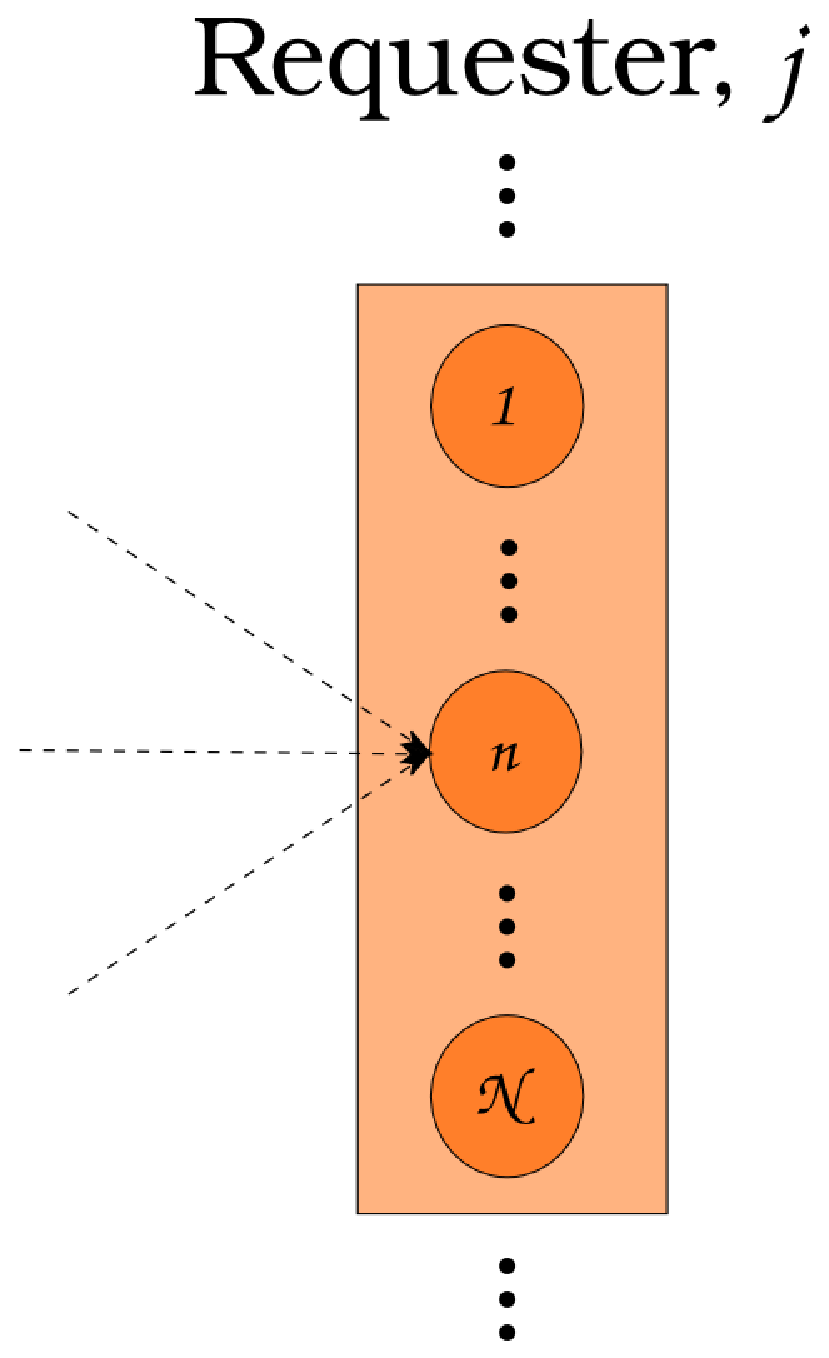
\includegraphics[height=5cm]{./images/requester.eps}
    \caption{Consumers define their demand for commodities during the Request
      for Bids (RFB) phase.}
  \end{figure}
\end{frame}

\begin{frame}[ctb!]
  \frametitle{Resource Exchange: Response to Request for Bids}
  \begin{figure}
    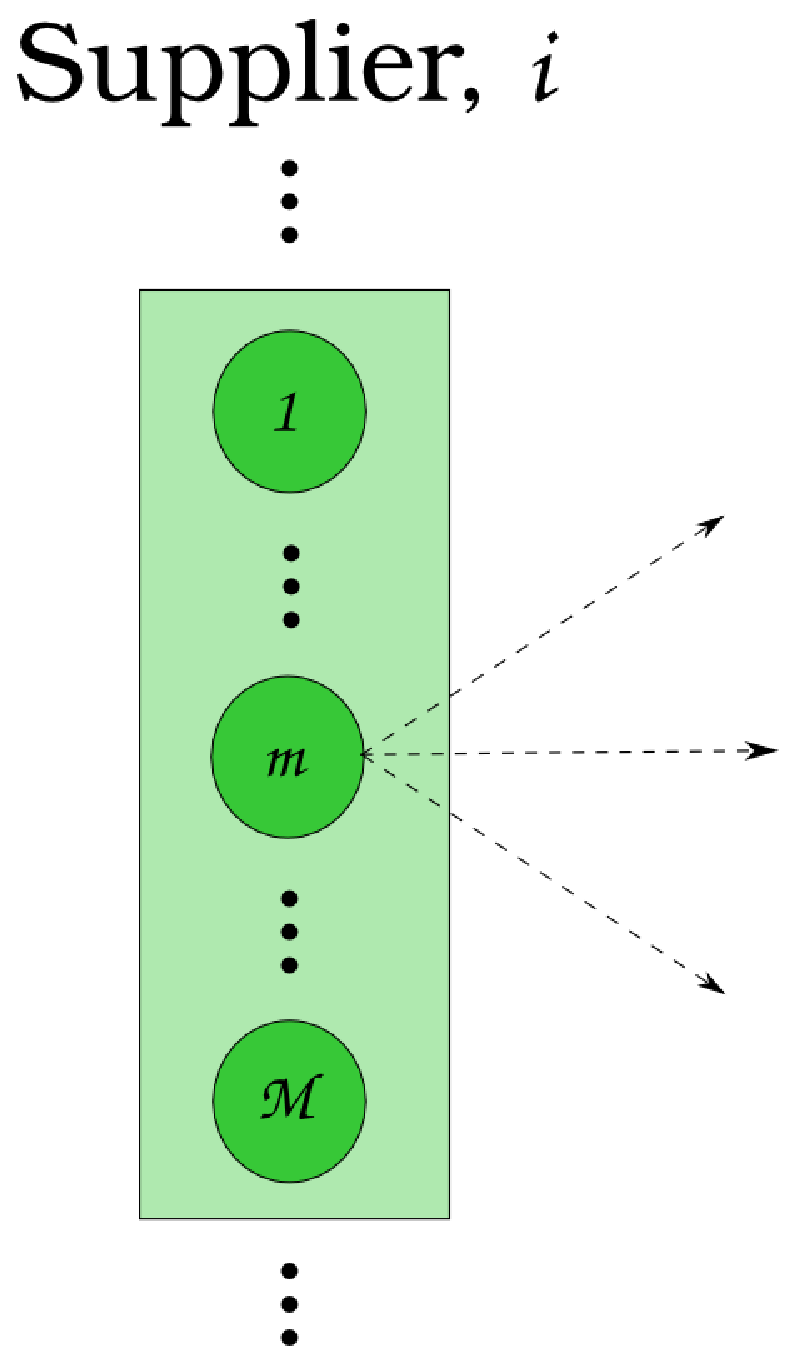
\includegraphics[height=5cm]{./images/supplier.eps}
    \caption{Suppliers respond to each request during the Response to Request
      for Bids (RRFB) phase.}
  \end{figure}
\end{frame}

\begin{frame}[ctb!]
  \frametitle{Resource Exchange: Preference Adjustment}
  \begin{figure}
    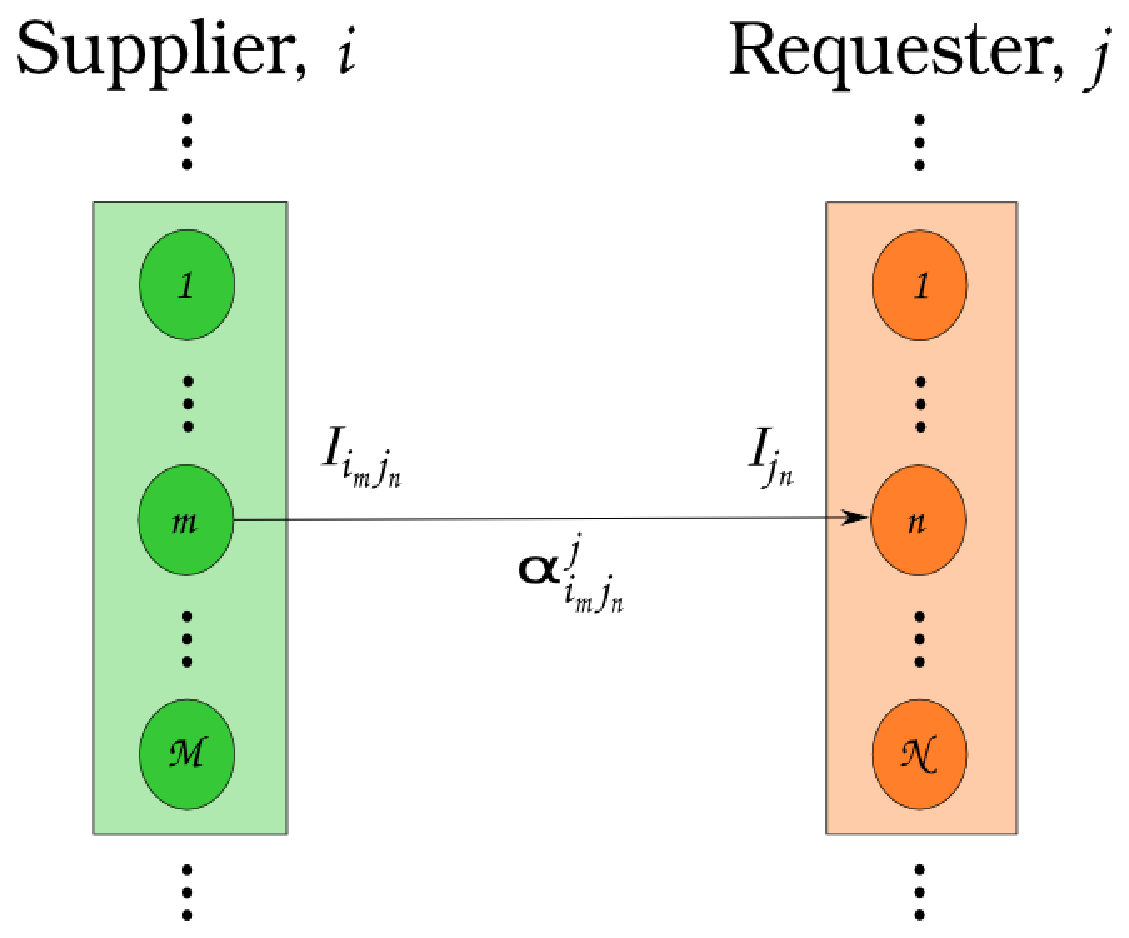
\includegraphics[height=4cm]{./images/supplier-requester.eps}
    \caption{Consumers adjust preferences based on Supplier-given information
      during the Preference Adjustment (PA) phase.}
  \end{figure}

  Managers of facilities (institutions, regions) are then allowed to perturb
  preferences.
\end{frame}

\begin{frame}[ctb!]
  \frametitle{Resource Exchange: Full Picture}
  \begin{figure}
    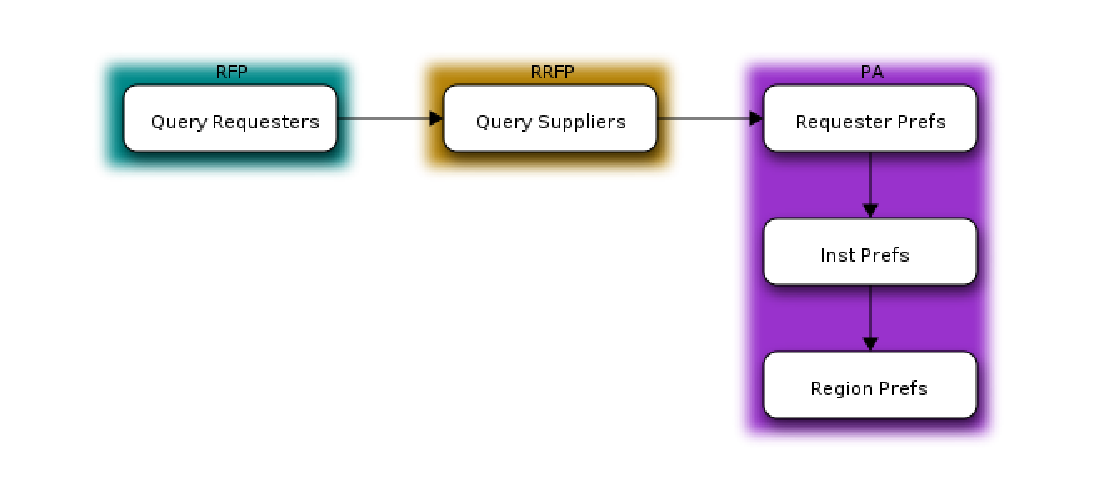
\includegraphics[height=5cm]{./images/exchange.eps}
    \caption{A flow chart of the information gathering phases.}
  \end{figure}
\end{frame}

\begin{frame}[ctb!]
  \frametitle{Resource Exchange Solution Mechanism}
  
  As defined, facilities in \Cyclus are black boxes, but there is a notion of
  supplier and consumer facilities of a variety of commodities.\vspace{0.2cm}

  We seek a solution to a flow of (discrete) materials, where for each
  commodity, we have now defined a set of suppliers and consumers of that
  commodity.\vspace{0.2cm} 
  
  Furthermore, suppliers may be able to provide more than one commodity and
  consumers may be able to consume more than one commodity.\vspace{0.2cm}

  Accordingly, a Multicommodity Transportation Problem formulation naturally
  fits the needs of our simulation. I have termed the formulation the Generic
  Fuel Cycle Transportation Problem (GFCTP).
  
\end{frame}

\begin{frame}[ctb!]
  \frametitle{GFCTP - Overview}
  
  The Generic Fuel Cycle Transportation problem assumes the following:

  \begin{itemize}
    \item there is a set of suppliers, a set of requesters, a set of
      commodities, and a set of possible resource transfers, defining arcs
      between suppliers and requesters
    \item a cardinal preference ordering if defined over the set of possible
      resource transfers
    \item suppliers can be constrained both by resource quantities and qualities
    \item multiple commodity types may satisfy a consumer
  \end{itemize}

\end{frame}
  

\begin{frame}[ctb!]
  \frametitle{GFCTP - Nomenclature}

  As we continue, I assume that the set of commodities is denoted $H$, the set
  of suppliers is denoted $I$, and the set of requesters is denoted $J$. The
  flow of commodity $h$ from supplier $i$ to consumer $j$ is denoted
  $x^h_{i,j}$.\vspace{0.2cm}

  I will first introduce the linear programming (LP) formulation, and then
  discuss its limitations when introducing the mixed integer-linear programming
  (MILP) formulation.

\end{frame}

\begin{frame}[ctb!]
  \frametitle{GFCTP (LP) - Request Constraint}
  
  A request can be met by multiple commodities in this framework. Take, for
  example, a reactor that can be supplied with two types of fuel, e.g. UOX and
  MOX.\vspace{0.2cm}

  Accordingly a consumer demands a set of commodities, $H_j$, and the total
  demand, $d_j$ must be met\footnote{A ``fake'' supplier with negative
    preference or infinite cost can be provided to avoid infeasibility},
  providing:

  \begin{equation}
    \sum_{i \in I}\sum_{h \in H_{j}} x_{i,j}^{h} \geq d_{j}(H_{j})  \: \forall j \in J
  \end{equation}
  
\end{frame}

\begin{frame}[ctb!]
  \frametitle{GFCTP (LP) - Supply Constraint - Example}
  
  A supplier of a commodity can meet multiple demands given constraints on its
  supply. There may be multiple constraints on supply, which may be a function
  of both quality and quantity of a requested commodity.\vspace{0.2cm}

  Take, for example, an enrichment facility that provides the commodity enriched
  uranium (ER). It may have multiple supply constraints, $s$, e.g.:
  \begin{itemize}
    \item A processing constraint, which has units of SWU
    \item An inventory constraint, which has units of kilograms of natural
      uranium (NU)
  \end{itemize}

\end{frame}

\begin{frame}[ctb!]
  \frametitle{GFCTP (LP) - Supply Constraint - Example}
  
  Given a request of ER at some enrichment level, $\varepsilon_j$, the
  constraints are defined as:

  \begin{equation}
    \sum_{j \in J} f_{SWU}(\varepsilon_j) x_{i,j}^{EU} \leq s_{i,SWU} 
  \end{equation}

  \begin{equation}
    \sum_{j \in J} f_{NU}(\varepsilon_j) x_{i,j}^{EU} \leq s_{i,NU} 
  \end{equation}

  \pause

  These constraints are a function of the isotopic profile of the request, or
  \textit{quality}, $q_j$. More generally suppliers may have conversion
  functions, which are functions of the request quality,
  $\beta_{i,k}(q_{j}^{h})$.

\end{frame}

\begin{frame}[ctb!]
  \frametitle{GFCTP (LP) - Supply Constraint}
  
  Assuming that a supplier may have $K$ different types of constraints for a
  commodity, $h$, the supply constraint is:

  \begin{equation}
    \sum_{j \in J}\beta_{i,k}(q_{j}^{h}) x_{i,j}^{h} \leq s_{i,k} 
    \: \forall \: k \in K_{i}^{h},  
    \forall \: i \in I, \forall \: h \in H
  \end{equation}

\end{frame}

\begin{frame}[ctb!]
  \frametitle{GFCTP (LP) - Objective Function}

  It is an open question whether the objective function should maximize
  preference or minimize an implied cost.\vspace{0.2cm}

  Because economics is a central metric, I believe that a general minimum cost
  architecture should be developed, and a preference-to-cost translation
  function should be used for the present time.\vspace{0.2cm}

  Assuming there is such a function, $f$, i.e.,
  \begin{equation}
    f : \alpha_{i,j}(h) \to c_{i,j}^{h}
  \end{equation}

  The the objective function is
  \begin{equation}
    \min \sum_{h \in H}\sum_{i \in I}\sum_{j \in J}c_{i,j}^{h} x_{i,j}^{h} 
  \end{equation}

\end{frame}

\begin{frame}[ctb!]
  \frametitle{GFCTP (LP) - Formulation} 

  With the normal non-negative flow constraint, the full GFCTP formulation is:
  
  %%%
  \begin{subequations}\label{eqs:GFCTP-LP}
    \begin{align}
      %%
      \min_{z} \:\: & 
      z = \sum_{h \in H}\sum_{i \in I}\sum_{j \in J}c_{i,j}^{h} x_{i,j}^{h} 
      & \label{eqs:GFCTP-LP_obj} \\
      %%
      \text{s.t.} \:\: &
      \sum_{j \in J}\beta_{i,k}(q_{j}^{h}) x_{i,j}^{h} \leq s_{i,k} 
      &
      \: \forall \: k \in K_{i}^{h},  
      \forall \: i \in I, \forall \: h \in H \label{eqs:GFCTP-LP_sup} \\
      %%
      &
      \sum_{i \in I}\sum_{h \in H_{j}} x_{i,j}^{h} \geq d_{j}(H_{j}) 
      & 
      \forall \: j \in J \label{eqs:GFCTP-LP_dem} \\
      %%
      &
      x^h_{i,j} \geq 0
      &
      \forall \: x \in X \label{eqs:GFCTP-LP_x}
      %%
    \end{align}
  \end{subequations}
  %%% 
\end{frame}

\begin{frame}[ctb!]
  \frametitle{GFCTP (LP) - Comments} 

  The LP formulation of the GFCTP is a fairly robust treatment of the proposed
  problem. It lacks robustness in one key area, though: order splitting.\vspace{0.2cm}

  Consider a thermal reactor's order constraint for UOX and MOX under the LP
  framework:

  \begin{equation}
    \sum_{i \in I} x_{i}^{MOX} + x_{i}^{UOX} \geq d(\{MOX,UOX\})
  \end{equation} 

  Such an order can be split by commodity and supplier. Given a solution,
  $x^{MOX}$, and $x^{UOX}$, the following values are possible:

  \begin{equation}
    x^{MOX} \in [0, d(\{MOX,UOX\})], \: x^{UOX} \in [0, d(\{MOX,UOX\})]
  \end{equation} 

\end{frame}

\begin{frame}[ctb!]
  \frametitle{GFCTP (MILP) - Overview}

  A tweaking of the LP formulation is provided to prevent order splitting. I
  assume that there is now a bipartite partition of consumers, those that
  require \textit{exclusive} orders, i.e., those that can not be split, and
  those allow \textit{partial}.

  \begin{equation}\label{eqs:consumer-union}
    J = J_{p} \cup J_{e}
  \end{equation}

  A binary variable is assigned to suppliers to guarantee that only one
  commodity from their demand set, $H_j$, is provided from a single supplier,
  $i$, i.e.,

  \begin{equation}
    \sum_{h \in H_j}\sum_{i \in I} y_{i,j}^{h} = 1
     \: \forall \: j \in J_{e}
  \end{equation}
  
\end{frame}

\begin{frame}[ctb!]
  \frametitle{GFCTP (MILP) - Request Constraint} 

  The MILP formulation now has two requests constraints, for each family of
  requests:

  \begin{equation}
    \sum_{i \in I}\sum_{h \in H_{j}} x_{i,j}^{h} \geq d_{j}(H_{j})
     \: \forall \: j \in J_{o}
  \end{equation}
  
  \begin{equation}    
    \sum_{i \in I}\sum_{h \in H_{j}} y_{i,j}^{h} \tilde{x}_{j}^{h} \geq d_{j}(H_{j}) 
     \: \forall \: j \in J_{e}
  \end{equation}

  The combination $y_{i,j}^{h} \tilde{x}_{j}^{h}$ is equivalent to the flow of
  commodity $h$ from supplier $i$ to requester $j$, $x^h_{i,j}$.
\end{frame}

\begin{frame}[ctb!]
  \frametitle{GFCTP (MILP) - Supply Constraint} 

  The MILP formulation supply constraints incorporate to two possible flows of
  material out of a supplier:
  
  \begin{equation}    
    \sum_{j \in J_{p}}\beta_{i,k}(q_{j}^{h}) x_{i,j}^{h}
    + \sum_{j \in J_{e}}\beta_{i,k}(q_{j}^{h}) y_{i,j}^{h} \tilde{x}_{j}^{h} \leq s_{i,k}^{h}
     \: \forall \: i \in I, \: \forall \: k \in K_{i}^{h}, \forall \: {h \in H}
  \end{equation}
  
\end{frame}

\begin{frame}[ctb!]
  \frametitle{GFCTP (MILP) - Formulation} 
  
  With a similar treatment of the objective function, the full formulation is:
  
  \begin{subequations}\label{eqs:GFCTP-E}
    \begin{align}
      %%
      \label{eq:GRCTP-E_obj}
      \min_{z} \:\: 
      & 
      z = \sum_{h \in H}\sum_{i \in I}\sum_{j \in J_{p}}c_{i,j}^{h} x_{i,j}^{h} 
      + \sum_{h \in H}\sum_{i \in I}\sum_{j \in J_{e}}c_{i,j}^{h} y_{i,j}^{h} \tilde{x}_{j}^{h}
      && \\
      %%
      \label{eq:GRCTP-E_sup}
      &
      \text{s.t.} \:\: 
      \sum_{j \in J_{p}}\beta_{i,k}(q_{j}^{h}) x_{i,j}^{h}
      + \sum_{j \in J_{e}}\beta_{i,k}(q_{j}^{h}) y_{i,j}^{h} \tilde{x}_{j}^{h} \leq s_{i,k}^{h} \nonumber \\
      &
      \qquad\qquad\qquad\qquad
      \forall \: i \in I, \: \forall \: k \in K_{i}^{h}, \forall \: {h \in H}\\
      %%
      \label{eq:GRCTP-E_dem_p}
      &
      \sum_{i \in I}\sum_{h \in H_{j}} x_{i,j}^{h} \geq d_{j}(H_{j})
      &
      \forall \: j \in J_{o} &\\
      %%
      \label{eq:GRCTP-E_dem_e}
      &
      \sum_{i \in I}\sum_{h \in H_{j}} y_{i,j}^{h} \tilde{x}_{j}^{h} \geq d_{j}(H_{j}) 
      &
      \forall \: j \in J_{e}  &\\
      %%
      \label{eq:GRCTP-E_sumy}
      &
      \sum_{h \in H}\sum_{i \in I} y_{i,j}^{h} = 1
      &
      \forall \: j \in J_{e}  &\\
      %%
      \label{eq:GRCTP-E_x}
      &
      x_{i,j}^{h} \geq 0
      &
      \forall \: x \in X  &\\
      %%
      \label{eq:GRCTP-E_y}
      &
      y_{i,j}^{h} \in \{0,1\}
      &
      \forall \: y \in Y &
      %%
    \end{align}
  \end{subequations}

\end{frame}

\begin{frame}[ctb!]
  \frametitle{Recipe Approximation Problem - Set Up} 

  Originally posed in a slightly different form by Oliver
  \cite{oliver_geniusv2:_2009}, the RAP assumes that a recycle fuel fabrication
  facility has a set of barrels of separated material.\vspace{0.2cm}

  Separated material is assumed to be separated by element (e.g. Pu) or by a
  group of elements (e.g. Am + Pu).\vspace{0.2cm}

  Each barrel is a homogeneous mixture of its isotopics, i.e., there is a barrel
  isotopic profile, $I_b$ and a barrel mass, $m_b$.\vspace{0.2cm}

  There are a series of orders, or target recipes, to fill, which similarly
  define an isotopic profile, $I_t$ and mass $m_t$.\vspace{0.2cm}

  Goal: Match the recipes as ``closely'' as possible.
\end{frame}

\begin{frame}[ctb!]
  \frametitle{Recipe Approximation Problem - Set Up} 
    \begin{figure}
    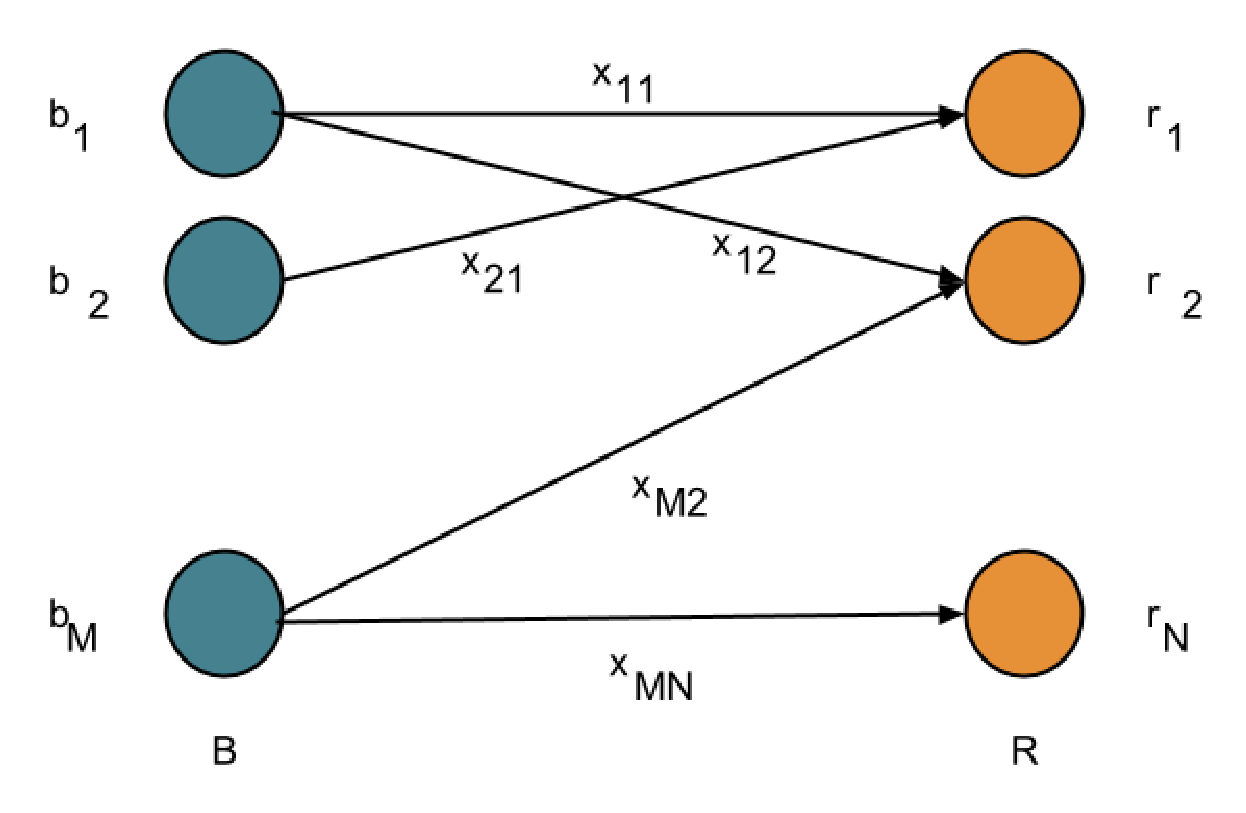
\includegraphics[height=5cm]{./images/rap.eps}
    \caption{A graphical view of the Recipe Approximation Problem.}
  \end{figure}
\end{frame}

\begin{frame}[ctb!]
  \frametitle{Recipe Approximation Problem - Set Up} 

  An $\ell_1$ norm approximation formulation is used, provided a target
  solution.\vspace{0.2cm}
  
  Properties of the determined solution comprise the objective and
  constraints.\vspace{0.2cm}

  The constraint properties are required to be met within some error, whereas
  the residual of the objective property is minimized.
\end{frame}

\begin{frame}[ctb!]
  \frametitle{Recipe Approximation Problem - Objective}

  In the current formulation, the matching the target recipe is the objective.

  Given a matrix of the barrel isotopic quantities, $M$, the residual between a
  possible solution and the target is defined as:
  
  \begin{equation}\label{eqs:residual}
    \vec{y_{t}} = \left| M \cdot \vec{x_{t}}  - m_t \vec{I_{t}} \right|.
  \end{equation}

  This sum of possible residuals is minimized, given a weighting factor, $c_t$:
  
  \begin{equation}\label{rap-obj}
    \min_{z} \:\: z = \sum_{t \in T} \vec{c_{t}}^{\top} \cdot \vec{y_{t}}
  \end{equation}
\end{frame}

\begin{frame}[ctb!]
  \frametitle{Recipe Approximation Problem - Objective Weights}

  A barrel may contain isotopics not present in a given target recipes.\vspace{0.2cm}

  Furthermore, certain isotopes, e.g. U-238, may dominate the mass of a
  recipe. However, their contribution to the running of a reactor may be
  relatively very low. Accordingly, the isotopic masses are weighted in a
  normalized manner, i.e.,

  \begin{equation}\label{eqs:weights}
    c_{i,t} = 
    \begin{cases}
      \frac{1}{m_{i,t}} & \text{if } i \in I_{t} \\
      \frac{1}{m_{t}}   & \text{if } i \not\in I_{t}
    \end{cases}
  \end{equation}  
\end{frame}

\begin{frame}[ctb!]
  \frametitle{Recipe Approximation Problem - Mass Constraint}

  A solution should be of approximately the same mass as the target. This
  constraint is required because of the normalization of the objective function.

  Given the mass of a possible solution, $m_{t^*}$, and a maximum violation,
  $\epsilon_{m}$, the constraint is
  
  \begin{equation}\label{eqs:mass-constraint-simple}
    \epsilon_{m} \geq \left| m_{t^*} - m_{t} \right|.
  \end{equation}
\end{frame}

\begin{frame}[ctb!]
  \frametitle{Recipe Approximation Problem - Neutronics Constraint}

  A solution should behave neutronically approximately the same as the
  target. The chosen parameter to constrain was the neutron reproduction factor,
  $eta$, due to its being a function solely of the recipe, rather than geometry
  or other reactor-specific parameters.

  $eta$ is defined for a homogeneous material as:

  \begin{equation}
    \label{eqs:eta_micro}
    \eta_t = \frac{\sum_{i \in I_t} \nu^{i} \sigma_{f}^{i} N^{i}}
        {\sum_{i \in I_t} \sigma_{a}^{i} N^{i}},
  \end{equation}

  with physical constants $\nu^{i}$, the average number of neutrons produced by
  fission of isotope $i$, $\sigma_{f}^{i}$, the microscopic fission cross
  section for isotope $i$, and $\sigma_{a}^{i}$, the microscopic absorption
  cross section for isotope $i$. $N^i$ is the number density for isotope $i$.
\end{frame}

\begin{frame}[ctb!]
  \frametitle{Recipe Approximation Problem - Neutronics Constraint}

  From the perspective of mixing of barrels, one can define the reproduction
  factor of a proposed solution as:

  \begin{equation}
    \label{eqs:eta_simple}
    \eta_{t^*} = \frac{\sum_{b \in B} \eta_{b}^{+} x_{b, t}}
        {\sum_{b \in B} \eta_{b}^{-} x_{b, t}}
  \end{equation}

  Where $\eta_b^+$ and $\eta_b^-$ are defined as:

  \begin{equation}
    \label{eqs:eta_+}
    \eta_{b}^{+} \equiv \sum_{i \in I_{b}} \nu^{i} \sigma_{f}^{i} N_{b}^{i}
  \end{equation}

  \begin{equation}
    \label{eqs:eta_-}
    \eta_{b}^{-} \equiv \sum_{i \in I_{b}} \sigma_{a}^{i} N_{b}^{i}
  \end{equation}
  
\end{frame}

\begin{frame}[ctb!]
  \frametitle{Recipe Approximation Problem - Neutronics Constraint} 

  This separation allows one to write the neutronics constraint, given a maximum
  possible violation, $\epsilon_{\eta}$, as:

  \begin{equation}
    \label{eqs:eta_linear}
    \epsilon_{\eta} \sum_{b \in B} \eta_{b}^{-} x_{b,t} \geq
    \left| \sum_{b \in B} \eta_{b}^{+} x_{b,t}
    - \eta_{t} \sum_{b \in B} \eta_{b}^{-} x_{b,t} \right|
  \end{equation}  
\end{frame}

\begin{frame}[ctb!]
  \frametitle{Recipe Approximation Problem - Formulation}

  The full formulation for the RAP is then:

  %%% 
  \begin{subequations}\label{eqs:rap}
    \begin{align}
      %%
      \min_{z} \:\: & 
      z = \sum_{t \in t} \vec{c_{t}}^{\top} \cdot \vec{y_{t}}
      & \label{eqs:rap_obj} \\
      %%
      \text{s.t.} \:\: &
      \vec{y_{t}} = \left| M \cdot \vec{x_{t}}  - m_t \vec{I_{t}} \right|
      &
      \: \forall \: t \in T \label{eqs:rap_iso} \\
      %%
      &
      \epsilon_{m} \geq \left| \sum_{b \in B} m_{b} x_{b, t} - m_{t} \right|
      & 
      \forall \: t \in T \label{eqs:rap_mass} \\
      %%
      &
      \epsilon_{\eta} \sum_{b \in B} \eta_{b}^{-} x_{b, t} \geq 
      \left| \sum_{b \in B} \eta_{b}^{+} x_{b, t} - 
      \eta_{t} \sum_{b \in B} \eta_{b}^{-} x_{b, t} \right|
      & 
      \forall \: t \in T \label{eqs:rap_eta} \\
      &
      \sum_{t \in T} x_{b, t} \leq 1
      & 
      \forall \: b \in B \label{eqs:rap_conserv} \\
      &
      x_{b, t} \in \left[ 0, 1 \right]
      & 
      \forall \: b \in B, \forall \: t \in T  \label{eqs:rap_x}
      %%
    \end{align}
  \end{subequations}
  %%% 
\end{frame}

\begin{frame}[ctb!]
  \frametitle{Recipe Approximation Problem - Research Questions} 

  Four primary research questions exist:

  \begin{enumerate}
    \item Does barrel size affect the accuracy of matches?
    \item Is isotopic ``closeness'' or neutronics parameter ``closeness'' the
      better objective function value?
    \item How to delineate between fast and thermal recipes?
    \item Are additional neutronics constraints helpful?
  \end{enumerate}
\end{frame}

\begin{frame}[ctb!]
  \frametitle{Next Steps} 
  
  The \Cyclus team has identified the one and two-tier fuel cycles proposed in
  the recent Dynamic Systems Analysis Report for Nuclear Fuel Recycle (DSARR)
  \cite{dixon_dynamic_2008} as targets for development.\vspace{0.2cm}

  The Information Gathering mechanism is required for a first-blush attempt at
  these cycles, as it provides a mechanism to determine basic preferential flow
  when there is more than one possible destination or source of
  material. Accordingly, it will be implemented first.\vspace{0.2cm}
\end{frame}

\begin{frame}[ctb!]
  \frametitle{Next Steps} 

  The LP formulation of the GFCTP will then be implemented for this simple
  case. Its capability will be demonstrated by providing preferences across
  institutions or regions. For example, servicing facilities (e.g. enrichment
  plants and separations facilities) can be either in the same institution or
  region as a reactor, and preferences can be assigned accordingly.\vspace{0.2cm}

  The MILP formulation for the GFCTP will then be implemented. Comparisons in
  run time and output will be observed, and, depending on outcomes, acceleration
  methods, such as cutting planes and preprocessing, will be investigated.\vspace{0.2cm}

  In both cases, the COIN-OR\cite{lougee_common_2003} suite of libraries will be
  used as the Simplex and Branch-and-Bound solvers.

\end{frame}

\begin{frame}[ctb!]
  \frametitle{Next Steps} 
  
  Finally, the RAP will be implemented in the simple simulation cases and
  compared with both the naive approach to fuel matching and the Equivalence
  Method as used in COSI. 

  Again, the COIN-OR Simplex solver will be leveraged to solve the RAP.

\end{frame}
